\documentclass[10pt,a4paper]{article}
\usepackage[margin=2.2cm]{geometry}
\usepackage[T1]{fontenc}
\usepackage[utf8]{inputenc}
\usepackage{lmodern,microtype}
\usepackage{amsmath,amssymb}
\usepackage{booktabs,array,tabularx}
\usepackage{graphicx,float}
\usepackage[font=small,labelfont=bf]{caption}
\usepackage{enumitem}
\setlist{nosep,leftmargin=1.4em}
\setlength{\parskip}{3pt}
\renewcommand{\arraystretch}{1.12}
\newcommand{\bpsHz}{bps/Hz}
\newcommand{\THT}{\boldsymbol{\Theta}}
\newcommand{\file}[1]{\texttt{\small #1}}

\begin{document}

\begin{center}
{\large\bfseries ECE 310 --- Wireless Communications --- Milestone 4 Report}\\[6pt]
{\Large\bfseries Quantifying the Sum-Rate Cost of Reciprocity in Beyond-Diagonal RIS-Aided MU-MISO Systems}\\[4pt]
{\large A Manifold-Optimisation Comparison Across Single-, Group- and Fully-Connected Architectures}\\[8pt]
Group 9 \quad|\quad Ahmedabad University\\[4pt]
Aashi Bhimjiyani (AU2440027) \quad Kahaan Shah (AU2440047)\\
Prakshal Shah (AU2440265) \quad Samridhi Mehrotra (AU2440033)\\[4pt]
November 14, 2026
\end{center}

\begin{abstract}\noindent
A lossless passive beyond-diagonal RIS (BD-RIS) has a unitary scattering matrix ($\THT^H\THT=\mathbf I$); if it is built from reciprocal components, $\THT$ must also be symmetric ($\THT=\THT^T$). This report quantifies the sum-rate lost to that extra constraint in a downlink MU-MISO system with a blocked direct link. A reciprocal design (Riemannian conjugate-gradient ascent with a symmetry penalty and an exact final symmetric-unitary projection) is compared with a general, non-reciprocal baseline on identical channels, start matrices and frozen MMSE precoders, so any rate difference is attributable to the symmetry constraint. Fifty-draw experiments cover transmit power, number of antennas and users, RIS size, group-connected block size and Rician fading, with diagnostics of the optimiser (iteration cap, penalty weight). The cost of reciprocity is exactly zero for single-connected (SC) RIS, between $0.10$ and $0.16$\,\bpsHz\ (1--9\,\% of the rate) for group-connected (GC) RIS with block size 4, and between $0.005$ and $0.11$\,\bpsHz\ (0.1--0.8\,\%) for fully-connected (FC) RIS at $N{=}K{=}2$. The GC cost grows strongly with the number of users ($0.59\to1.68$\,\bpsHz\ for $N{=}K{=}3\to6$), shrinks as the GC block size grows, and is largely independent of $R$. Reciprocity is therefore nearly free when the RIS blocks are large compared with $N{+}K$ and costly when they are small. Some low-power results are partly optimiser-limited, and the report states which.
\end{abstract}

\section{Introduction and problem formulation}
\subsection{Motivation}
Conventional RIS uses a diagonal scattering matrix, so each element reflects independently. BD-RIS permits a non-diagonal, inter-connected scattering matrix, which adds degrees of freedom and raises the achievable sum rate, at the price of more circuit complexity. Its architectures differ in how the elements are connected: single-connected (SC, diagonal), group-connected (GC, block-diagonal) and fully-connected (FC, full matrix). A passive lossless BD-RIS built only from reciprocal components must have a symmetric scattering matrix, whereas unconstrained unitary designs ignore this and generally require non-reciprocal (active) hardware. The question studied here is how much sum rate is lost by enforcing reciprocity.

\subsection{System model}
A BS with $N$ antennas serves $K$ single-antenna users through an $R$-port lossless BD-RIS; the direct link is blocked:
\[
\mathbf r=\mathbf H_{RX}\,\THT\,\mathbf H_{TX}\,\mathbf V\mathbf s+\mathbf n,\qquad
\mathbf H_{TX}\in\mathbb C^{R\times N},\ \mathbf H_{RX}\in\mathbb C^{K\times R},\ \mathbf V\in\mathbb C^{N\times K},\ \|\mathbf V\|_F^2\le P_{\max}.
\]
With $\mathbf e_k$ the $k$-th row of $\mathbf E=\mathbf H_{RX}\THT\mathbf H_{TX}$ and $c_{ki}=\mathbf e_k\mathbf v_i$, the SINR is $\gamma_k=|c_{kk}|^2/(\sum_{i\ne k}|c_{ki}|^2+N_0)$ and the sum rate is $R_{\rm sum}=\sum_k\log_2(1+\gamma_k)$. Path loss is $C(d/d_0)^{-\alpha}$ with $C=-30$\,dB, $\alpha=2.2$, BS--RIS distance 50\,m, RIS--user distance 2.5\,m, noise $-80$\,dBm; fading is Rayleigh or Rician.

\subsection{Feasible sets and the research question}
The general design requires $\THT^H\THT=\mathbf I$ with the block structure of the chosen architecture; the reciprocal design additionally requires $\THT=\THT^T$.
\begin{table}[H]\centering\small
\begin{tabular}{@{}lccc@{}}\toprule
Architecture & Structure & General real DoF & Reciprocal real DoF\\\midrule
SC & diagonal & $R$ & $R$\\
GC & $G$ blocks, $R_g=R/G$ & $G R_g^2$ & $G R_g(R_g{+}1)/2$\\
FC & one $R\times R$ block & $R^2$ & $R(R{+}1)/2$\\\bottomrule
\end{tabular}
\end{table}
A diagonal unitary matrix is already symmetric, so \emph{SC is an exact zero-gap control}. The \textbf{reciprocity gap} is $\Delta R=R_{\rm general}-R_{\rm reciprocal}$ under a common frozen MMSE precoder (positive: reciprocity costs rate). The research question is how large $\Delta R$ is for SC, GC and FC and how it depends on power, number of users, RIS size, group size and fading.

\section{Related work}
\textbf{BD-RIS architectures and joint design.} Li, Shen and Clerckx~[1] introduce a unified BD-RIS framework covering reflective, transmissive and hybrid modes and the single-, group- and fully-connected architectures, together with joint transmit-precoder/BD-RIS optimisation for sum-rate maximisation based on fractional programming~[6] and Riemannian optimisation~[7]. Their formulation does not impose reciprocity and is not a matched study of the reciprocity gap; we use it as the general baseline.

\textbf{Scattering-network modelling.} Shen, Clerckx and Murch~[5] model RIS hardware through scattering-parameter network analysis; for a passive lossless reciprocal network this gives the unitary and symmetric scattering matrix used here.

\textbf{Reciprocal BD-RIS design.} Recent work designs reciprocal (symmetric-unitary) BD-RIS scattering matrices by manifold optimisation~[2]--[4]. Reference~[2] enforces reciprocity with a penalty; reference~[3] reports reciprocal and general curves that nearly coincide; reference~[4] studies the geometry of symmetric-unitary matrices and a low-rank property. These works motivate the question asked here, but they do not report a matched, paired measurement of the gap with confidence intervals across architectures and operating conditions, which is what this project provides.

\section{Proposed methodology}
\subsection{Matched-comparison protocol}
For each draw $d$, both designs receive the same channels (\texttt{rng(seed\_base+d)}), the same start matrix (the shared diagonal SC matrix), and the same initial MMSE precoder $\mathbf V_0$. The precoder is frozen, so the two designs differ only in the symmetry constraint. Every reported rate is recomputed with the common SINR/sum-rate functions on the final (projected) matrices.

\subsection{Reciprocal design}
\begin{enumerate}
\item Fractional programming (Lagrangian dual and quadratic transform) turns the sum rate into a surrogate in $\THT$ with auxiliary variables refreshed after every accepted step.
\item The objective is $F_{\rm FP}(\THT)-\nu\|\THT-\THT^T\|_F^2$ with $\nu=1$; the analytic gradient includes the penalty term and matches central finite differences to relative error $\le4.6\times10^{-9}$ for $R_g\in\{1,4,32\}$.
\item Riemannian gradient by tangent projection onto the (block) unitary manifold; Polak--Ribi\`ere conjugate direction with reset; Armijo backtracking; SVD-polar retraction.
\item Stopping: surrogate change below $10^{-8}$ or 8000 iterations (configurable).
\item Exact enforcement: symmetrise each block, $\THT_{\rm sym}=\tfrac12(\THT_g+\THT_g^T)$, then take the unitary polar factor via SVD. The polar factor of a symmetric matrix is symmetric, so the result is exactly unitary and symmetric ($\approx10^{-14}$). The projection costs about $10^{-3}$\,\bpsHz\ on average at the anchor.
\end{enumerate}

\subsection{General baseline}
The matched, $\mathbf V$-frozen baseline (\texttt{general\_fixedV\_optimizer}) uses the same optimiser with $\nu=0$ and a plain block-unitary projection, following Li et al.~[1] (reflective mode). It differs from the reciprocal method only in the symmetry constraint. Li's joint $(\mathbf V,\THT)$ block-coordinate algorithm (\texttt{li\_joint\_optimizer}) is kept as a separate reference ceiling.

\section{Implementation}
All code is in \file{M4\_Group9/Code/src} (MATLAB, base functionality only). A single configuration (\file{configs/default\_config.m}), one channel generator, one start-matrix routine, one MMSE precoder and one SINR/sum-rate implementation (\file{common/}) are shared by both pipelines; \file{reciprocal/} holds the reciprocal optimiser and \file{nonreciprocal/} the general baseline and Li's joint design. The matched runner stores per-draw rates, iteration counts, run times and feasibility errors, with per-draw checkpointing and full-configuration matching. Experiment drivers in \file{experiments/} run each sweep, \file{analyze\_gap.m} computes the gap statistics (mean $\pm$ SE, 95\,\% bootstrap CI, medians, win counts, cap hits) from the per-draw files, and \file{make\_figures.m} produces the figures. The iteration cap is configurable (\texttt{p.max\_iter}); tests under \file{tests/} check parity between the common framework and the reciprocal code, reproducibility of seeds and the anchor statistics.

\section{Experimental setup}
\begin{table}[H]\centering\small
\begin{tabular}{@{}ll@{}}\toprule
Quantity & Value\\\midrule
Anchor condition & Rayleigh, $N{=}K{=}2$, $R{=}32$ ($G{=}8$, $R_g{=}4$), $P_{\max}=20$\,dBm, $N_0=-80$\,dBm\\
Sweeps (one factor varied) & $P_{\max}\in\{0,5,10,15\}$\,dBm; $N{=}K\in\{3,4,6\}$; $R\in\{16,48,64\}$ ($R_g{=}4$); $R_g\in\{2,8,16\}$ at $R{=}32$; Rician $K_f=2$\,dB\\
Draws & 50 per condition, seeds $1$--$50$ (identical across conditions)\\
Optimiser & $\nu=1$, tolerance $10^{-8}$, 8000-iteration cap, $\mathbf V$ frozen to the MMSE precoder at the start matrix\\\bottomrule
\end{tabular}
\end{table}
\textbf{Metric.} Per-draw gap $\Delta R=R_{\rm general,fv}-R_{\rm reciprocal,fv}$, reported as mean $\pm$ standard error with a 95\,\% percentile-bootstrap CI of the paired mean (4000 resamples, fixed seed), computed by the same script for every condition. Percentages are ratios of means (mean gap / mean general rate). A draw is a win for a design if its rate is higher by more than $10^{-9}$\,\bpsHz. Negative gaps are kept, not clipped: both designs stop at local optima, and a general optimum can never truly lie below a reciprocal one.

\section{Results}
\subsection{Anchor and Rician conditions}
\begin{table}[H]\centering\small
\begin{tabular}{@{}llrrrrrr@{}}\toprule
Fading & Arch. & Recip.\ rate & Gap $\pm$ SE & 95\,\% CI & Gap (\%) & Gen./Rec.\ better & Rec.\ cap hits\\\midrule
Rayleigh & SC & 8.517 & 0 & -- & 0 & 0/0 & 0\\
Rayleigh & GC & 9.909 & $0.103\pm0.026$ & [0.055, 0.155] & 1.03 & 48/2 & 4\\
Rayleigh & FC & 10.310 & $0.021\pm0.012$ & [0.001, 0.045] & 0.20 & 43/7 & 0\\\addlinespace
Rician 2\,dB & SC & 9.001 & 0 & -- & 0 & 0/0 & 0\\
Rician 2\,dB & GC & 10.346 & $0.085\pm0.038$ & [0.005, 0.154] & 0.81 & 46/4 & 8\\
Rician 2\,dB & FC & 10.683 & $0.037\pm0.018$ & [0.007, 0.078] & 0.35 & 46/4 & 1\\\bottomrule
\end{tabular}
\caption{Anchor ($N{=}K{=}2$, $R{=}32$, 20\,dBm), 50 draws, rates in \bpsHz.}
\end{table}
The Rician and Rayleigh gaps have overlapping confidence intervals, so no fading effect on the gap can be claimed; fading changes the rate level (SC: 8.52 vs 9.00\,\bpsHz) far more than the gap.

\subsection{Transmit power}
\begin{table}[H]\centering\small
\begin{tabular}{@{}rrrrrrrr@{}}\toprule
 & \multicolumn{4}{c}{GC ($R_g{=}4$)} & \multicolumn{3}{c}{FC}\\\cmidrule(lr){2-5}\cmidrule(lr){6-8}
$P_{\max}$ (dBm) & Gap $\pm$ SE & 95\,\% CI & \% & Rec.\ cap hits & Gap $\pm$ SE & \% & Rec.\ FC rate\\\midrule
0  & $0.148\pm0.028$ & [0.103, 0.207] & 9.36 & 30/50 & $0.0096\pm0.0018$ & 0.54 & 1.77\\
5  & $0.156\pm0.010$ & [0.138, 0.176] & 5.22 & 22/50 & $0.0170\pm0.0029$ & 0.51 & 3.29\\
10 & $0.147\pm0.017$ & [0.115, 0.179] & 3.02 & 11/50 & $0.0051\pm0.0022$ & 0.10 & 5.13\\
15 & $0.125\pm0.022$ & [0.084, 0.168] & 1.74 & 2/50  & $0.0067\pm0.0057$ & 0.09 & 7.47\\
20 & $0.103\pm0.026$ & [0.055, 0.155] & 1.03 & 4/50  & $0.0209\pm0.0116$ & 0.20 & 10.31\\\bottomrule
\end{tabular}
\caption{Power sweep (gaps in \bpsHz; 20\,dBm is the anchor).}
\end{table}
The absolute GC gap is almost flat in power (0.10--0.16\,\bpsHz) while the sum rate grows from 1.6 to 10\,\bpsHz, so the \emph{relative} cost falls from 9.4\,\% to 1.0\,\%. Low power is where reciprocity matters most, and also where the reciprocal optimiser most often reaches its iteration cap (Section~6.6).

\subsection{Number of antennas and users}
\begin{table}[H]\centering\small
\begin{tabular}{@{}rrrrrrrr@{}}\toprule
 & \multicolumn{4}{c}{GC ($R_g{=}4$)} & \multicolumn{3}{c}{FC}\\\cmidrule(lr){2-5}\cmidrule(lr){6-8}
$N{=}K$ & Gap $\pm$ SE & 95\,\% CI & \% & Rec.\ cap hits & Gap $\pm$ SE & 95\,\% CI & \%\\\midrule
2 & $0.103\pm0.026$ & [0.055, 0.155] & 1.03 & 4 & $0.021\pm0.012$ & [0.001, 0.045] & 0.20\\
3 & $0.591\pm0.044$ & [0.513, 0.680] & 5.26 & 5 & $0.085\pm0.023$ & [0.047, 0.134] & 0.71\\
4 & $1.068\pm0.073$ & [0.918, 1.197] & 9.25 & 1 & $0.110\pm0.024$ & [0.065, 0.162] & 0.87\\
6 & $1.683\pm0.061$ & [1.571, 1.801] & 14.78 & 0 & $0.292\pm0.039$ & [0.223, 0.374] & 2.05\\\bottomrule
\end{tabular}
\caption{Antenna/user sweep at 20\,dBm, $R{=}32$.}
\end{table}
For GC the gap increases roughly linearly with $N{=}K$ and reaches 15\,\% of the rate at $N{=}K{=}6$; it exceeds the FC gap by an order of magnitude. Cap hits are rare, so this result is not caused by the optimiser stopping early.

\subsection{RIS size}
\begin{table}[H]\centering\small
\begin{tabular}{@{}rrrrrrrr@{}}\toprule
 & \multicolumn{4}{c}{GC ($R_g{=}4$)} & \multicolumn{3}{c}{FC}\\\cmidrule(lr){2-5}\cmidrule(lr){6-8}
$R$ & Gap $\pm$ SE & 95\,\% CI & \% & Rec./Gen.\ cap hits & Gap $\pm$ SE & 95\,\% CI & \%\\\midrule
16 & $0.140\pm0.023$ & [0.097, 0.187] & 2.06 & 4/0 & $0.015\pm0.009$ & [0.001, 0.034] & 0.21\\
32 & $0.103\pm0.026$ & [0.055, 0.155] & 1.03 & 4/0 & $0.021\pm0.012$ & [0.001, 0.045] & 0.20\\
48 & $0.155\pm0.026$ & [0.105, 0.208] & 1.25 & 12/3 & $0.043\pm0.024$ & [0.003, 0.094] & 0.34\\
64 & $0.155\pm0.043$ & [0.078, 0.245] & 1.16 & 5/2 & $0.113\pm0.042$ & [0.044, 0.206] & 0.82\\\bottomrule
\end{tabular}
\caption{RIS-size sweep, $N{=}K{=}2$, 20\,dBm.}
\end{table}
At fixed block size 4 the GC gap shows no trend with $R$ (0.10--0.16\,\bpsHz, intervals overlap). The FC gap rises at $R{=}64$, but there the general solver itself reached the cap in 4 FC draws, which understates the gap, and 6 FC draws show a negative gap (down to $-0.19$\,\bpsHz); an FC trend with $R$ is not established. Excluding capped draws moves the GC gap from 0.155 to 0.139\,\bpsHz\ at $R{=}48$ and from 0.155 to 0.140\,\bpsHz\ at $R{=}64$.

\subsection{GC block size}
\begin{table}[H]\centering\small
\begin{tabular}{@{}rrrr@{}}\toprule
GC block size $R_g$ ($G$) & Reciprocal rate & General rate & Mean gap (\bpsHz)\\\midrule
2 (16) & 9.2485 & 9.5865 & 0.3380\\
4 (8) --- anchor & 9.909 & 10.012 & 0.103\\
8 (4) & 10.1824 & 10.2081 & 0.0258\\
16 (2) & 10.2588 & 10.2816 & 0.0228\\\bottomrule
\end{tabular}
\caption{GC block-size sweep, Rayleigh, $R{=}32$, $N{=}K{=}2$, 50 draws.}
\end{table}
The gap falls monotonically as the GC block grows, from 0.34\,\bpsHz\ at $R_g=2$ to $\approx0.02$\,\bpsHz\ for $R_g\ge8$.

\subsection{Optimiser diagnostics}
\textbf{Iteration cap (10 GC draws, 8000 vs.\ 40\,000 iterations; four draws that hit the cap at the anchor, six ordinary).} Raising the cap changes the reciprocal rate by $+0.0048$\,\bpsHz\ on the four capped draws and by $+0.0019$\,\bpsHz\ over all ten; the gap moves from 0.204 to 0.199\,\bpsHz\ on the capped draws. Three of the four capped draws converge below 40\,000 iterations. At 20\,dBm the cap therefore distorts the rate by $<0.005$\,\bpsHz. This check was run at 20\,dBm; at 0--10\,dBm the reciprocal GC optimiser reaches the cap in 30, 22 and 11 of 50 draws, so the low-power GC gaps may include optimiser error and the near-constant absolute gap in power should be read with that in mind.

\textbf{Penalty weight $\nu\in\{0.1,1,10\}$ (20 draws, GC and FC).} For GC the three reciprocal rates (9.240, 9.207, 9.241\,\bpsHz) are statistically indistinguishable (paired $\nu{=}1$ minus $\nu{=}0.1$: $-0.032\pm0.050$). $\nu{=}10$ makes the penalty gradient stiff: 7 of 20 GC draws reach the cap, against 0 for $\nu{=}1$. For FC, $\nu{=}1$ and $\nu{=}10$ give identical rates and avoid the projection loss of $\nu{=}0.1$ (0.018\,\bpsHz). A four-seed, 25\,000-iteration subset gives GC gaps of 0.044, 0.272 and 0.036\,\bpsHz\ for $\nu=0.1,1,10$; with four draws this is dominated by one seed. We therefore treat $\nu{=}1$ as an adequate engineering default, not as an optimum.

\textbf{A premature stop in the anchor run.} Draw 11 (GC) stops after 27 iterations because the surrogate change falls below $10^{-8}$, leaving a gap of 0.932\,\bpsHz; the same channel under $\nu=0.1$ or 10 gives 0.037 and 0.013\,\bpsHz. This single draw contributes about 0.019\,\bpsHz\ (roughly 18\,\%) of the 0.103\,\bpsHz\ anchor GC gap. It is kept in all tables (no post-hoc exclusion).

\textbf{Power convention.} Raising $P_{\max}$ to 23\,dBm tests whether the 20\,dBm reciprocal FC rate (10.31\,\bpsHz) is lower than the $\approx14$\,\bpsHz\ of the source paper's FC curve because the paper uses a total-power budget. The reciprocal FC rate rises to 12.17\,\bpsHz\ with gaps GC $0.101\pm0.019$ and FC $0.023\pm0.012$\,\bpsHz\ (unchanged from 20\,dBm), so the convention explains part of the difference. No parameter was tuned.

\subsection{Validation of the implementation}
\begin{table}[H]\centering\small
\begin{tabularx}{\textwidth}{@{}>{\raggedright\arraybackslash}p{4.1cm}Xl@{}}\toprule
Check & Evidence & Status\\\midrule
Framework parity (config, channels, start matrix, MMSE, SINR, rate, seeds, power budget, overrides) & \file{tests/test\_common\_framework.m}: all checks pass, re-run on the final code via \file{m4\_smoke\_test} & PASS\\
General baseline (surrogate $=$ eq.\ (21a) of~[1] to $1.4\times10^{-14}$, gradient FD error $\le3.7\times10^{-9}$, monotone ascent, unitarity $\approx10^{-15}$, block structure) & \file{test\_general\_baseline.m}, record in \file{Results/diagnostics/baseline\_validation} & 12/12 PASS\\
Reciprocal gradient & relative error $2.3\times10^{-9}$, $1.8\times10^{-9}$, $4.5\times10^{-9}$ for $R_g=1,4,32$ & PASS\\
Feasibility & reciprocal symmetry/unitarity error $\le1.5\times10^{-14}$ in every sweep; general unitarity $\le6\times10^{-15}$ & PASS\\
SC zero-gap control & gap exactly 0, 50/50 ties in all 13 conditions & PASS\\
Qualitative trends of~[1] (rate grows with power; FC$\ge$GC$\ge$SC) & 20 draws, $N{=}K{=}4$, joint design (hence higher rates, e.g.\ FC 22.97\,\bpsHz\ at 20\,dBm, than the frozen-$\mathbf V$ anchor) & PASS\\
Anchor statistics & \file{tests/test\_analyze\_gap\_anchor.m}: means, bootstrap CIs and win counts match M3 & PASS\\\bottomrule
\end{tabularx}
\end{table}

\section{Baseline comparison}
\begin{table}[H]\centering\small
\begin{tabular}{@{}lp{4.6cm}p{5.8cm}@{}}\toprule
Baseline & Definition & Role and result at the anchor\\\midrule
General, $\mathbf V$-frozen & same optimiser, $\nu=0$, unitary projection & Primary comparator. Rates 8.52 / 10.01 / 10.33\,\bpsHz\ (SC / GC / FC)\\
Reciprocal (proposed) & penalty + exact symmetric-unitary projection & 8.52 / 9.91 / 10.31\,\bpsHz; retains 99.0\,\% (GC) and 99.8\,\% (FC) of the general rate\\
SC control & diagonal matrix & Gap exactly 0 in all conditions; confirms the pipeline\\
Recomputed-$\mathbf V$ gap & MMSE recomputed at final $\THT$ & GC 0.126, FC 0.021\,\bpsHz; same picture as frozen $\mathbf V$\\
Li joint design~[1] & updates $\mathbf V$ and $\THT$ & Reference ceiling: 11.29 / 13.10 / 13.71\,\bpsHz, about 2.8--3.4\,\bpsHz\ above the frozen-$\mathbf V$ values; the improvement comes from updating $\mathbf V$, not from reciprocity\\\bottomrule
\end{tabular}
\end{table}
Under the DoF count of Section~1.3, the reciprocal GC design (block size 4) uses 62.5\,\% and the reciprocal FC design 51.6\,\% of the degrees of freedom of the general design, yet retains 99.0\,\% and 99.8\,\% of its rate at the anchor; the fixed-$\mathbf V$ ordering SC $<$ GC $<$ FC holds for both designs. Relative to the closest literature~[1]--[4], the added value is a matched paired comparison under a common precoder with an exact zero control and confidence intervals; Li et al.\ do not impose reciprocity, and the reciprocal-design papers report curves rather than paired gaps.

\begin{figure}[H]\centering
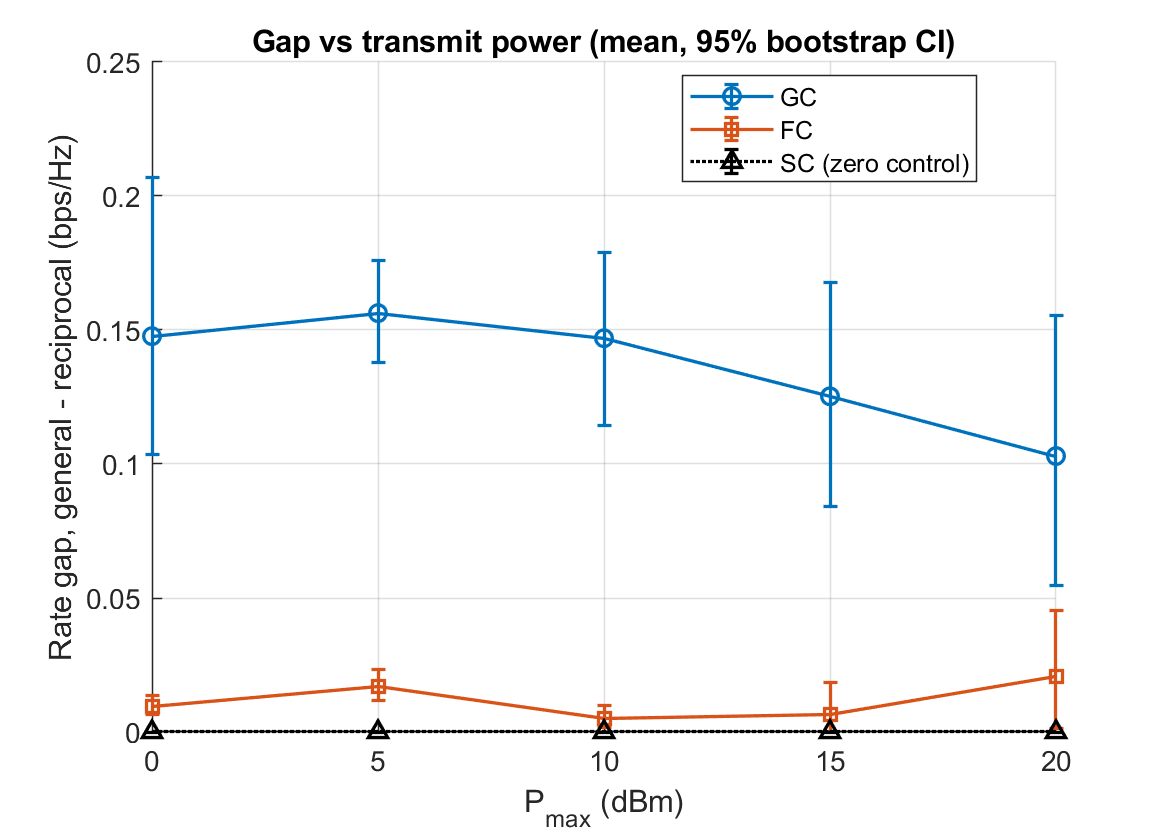
\includegraphics[width=0.48\textwidth]{figures/gap_vs_power.png}\hfill
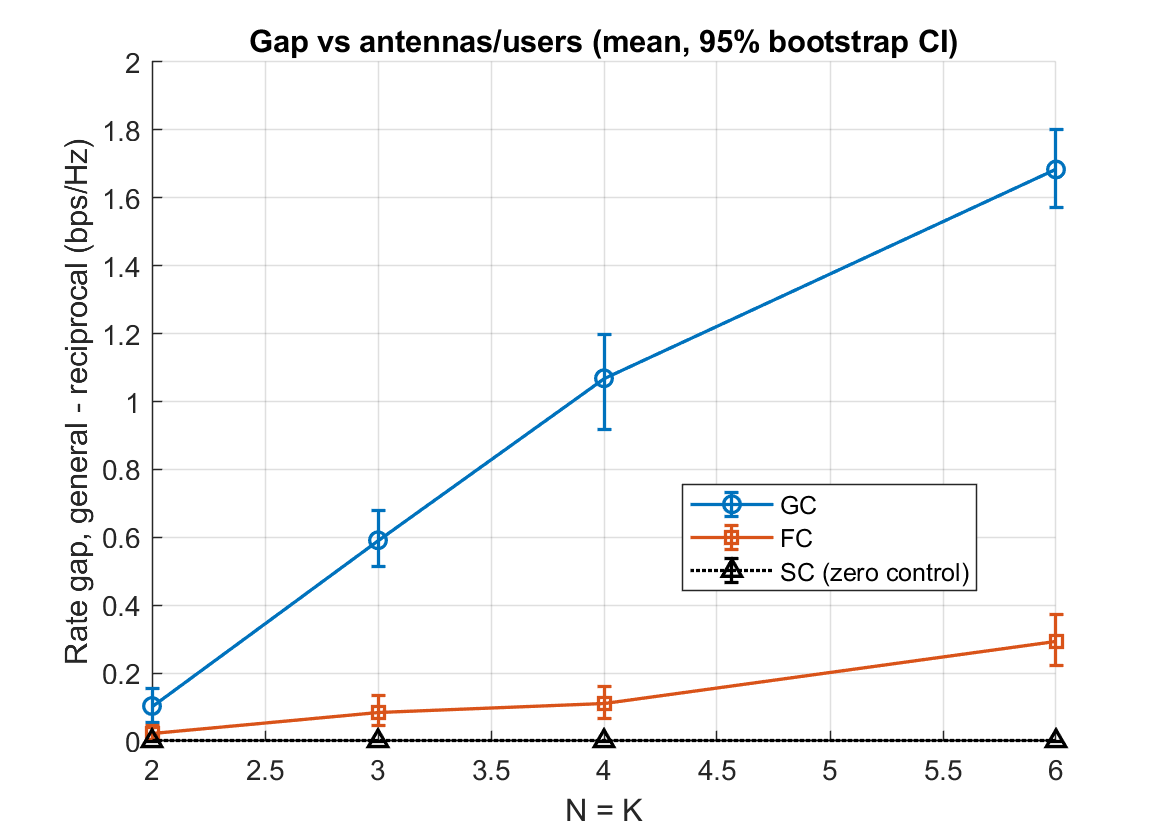
\includegraphics[width=0.48\textwidth]{figures/gap_vs_NK.png}\\[4pt]
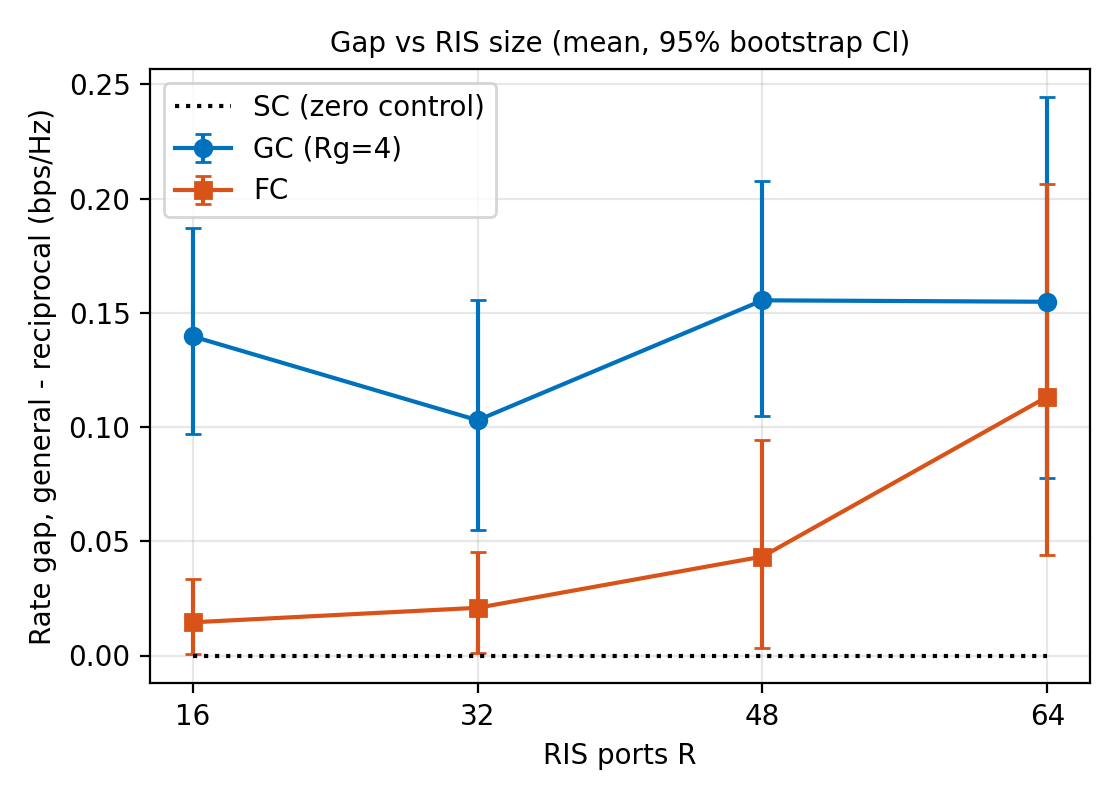
\includegraphics[width=0.48\textwidth]{figures/gap_vs_R.png}\hfill
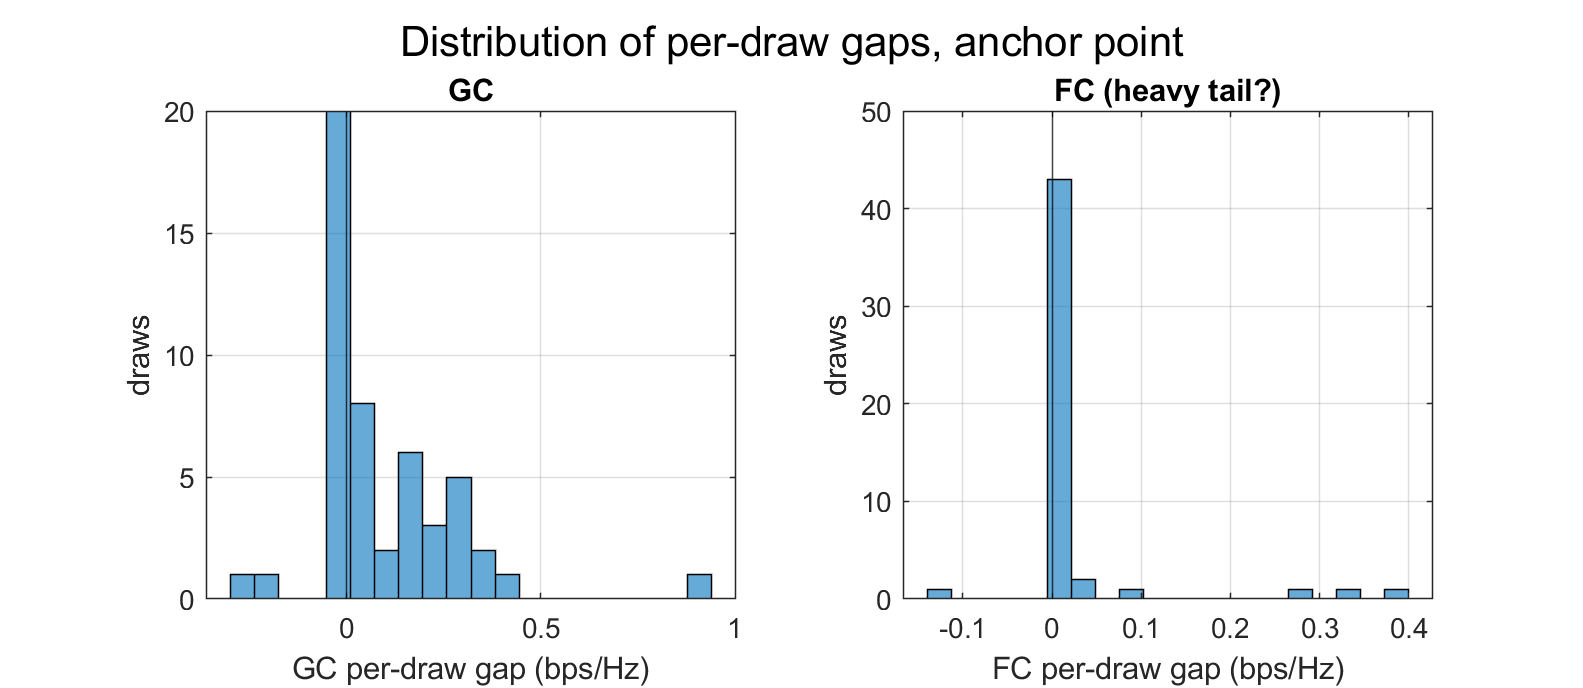
\includegraphics[width=0.48\textwidth]{figures/gap_distribution_anchor.png}
\caption{Reciprocity gap against transmit power (top left), $N{=}K$ (top right), RIS size $R$ (bottom left) and the per-draw gap distribution at the anchor (bottom right). Error bars are 95\,\% bootstrap CIs.}
\end{figure}

\section{Critical analysis}
\textbf{What the evidence supports.} (i) SC is exactly zero, confirming the pipeline. (ii) The GC cost is positive in 46--50 of 50 draws in every condition with a CI that excludes zero. (iii) The FC cost is small ($\le0.9$\,\% at $N{=}K=2$) but positive in each condition. (iv) The cost depends strongly on the number of users and on the GC block size, and weakly on $R$, on absolute power and on fading.

\textbf{Block size against $N{+}K$.} Three independent sweeps point the same way. With $R_g=4$ fixed, increasing $N{=}K$ (so $N{+}K$ grows past the block size) raises the GC gap from 0.10 to 1.68\,\bpsHz. At fixed $N{=}K{=}2$, increasing $R_g$ from 2 to 16 lowers it from 0.34 to 0.02\,\bpsHz. Changing $R$ at fixed $R_g$ and $N{=}K$ leaves it roughly unchanged. A symmetric block has $R_g(R_g+1)/2$ real degrees of freedom against $R_g^2$ for a general one; when a block is large compared with the $N{+}K$ streams it serves, the symmetric set still contains good solutions, and when it is not, symmetry binds. This explanation fits all tested points and the low-rank property of symmetric-unitary matrices~[4]; it has not been tested directly (for example by an $R_g$ sweep at $N{=}K{=}4$) and is offered as a consistent picture, not a proof. It also explains why FC loses less than GC at $N{=}K{=}2$.

\textbf{Where the numbers need care.}
\begin{itemize}
\item \emph{Optimiser against constraint.} Cap hits are frequent at low power (reciprocal GC 30/50 at 0\,dBm) and at $R{=}48$ (12/50), and the 40\,000-iteration check exists only at 20\,dBm and $R{=}32$. The GC gaps at 0--10\,dBm and $R{=}48$ may include optimiser error; the $N{=}K$ results do not (0--5 hits).
\item \emph{Premature stop.} One anchor draw contributes about 18\,\% of the anchor GC gap (Section~6.6).
\item \emph{Negative gaps} occur in 0--8 of 50 draws per condition (mostly FC). They reflect local optima and are retained.
\item \emph{Frozen precoder.} The primary gap holds $\mathbf V$ fixed. The recomputed-$\mathbf V$ gap is reported alongside and agrees; the joint design is a reference only.
\item \emph{Reproduction gap.} The reciprocal FC rate (10.31\,\bpsHz, frozen $\mathbf V$) is below the $\approx14$\,\bpsHz\ of the source paper's FC curve; the power-convention check narrows but does not close this, and no parameter was tuned.
\end{itemize}

\section{Limitations}
\begin{itemize}
\item Penalty plus projection is the only enforcement method studied, so the reciprocity cost and the quality of its enforcement are not fully separated.
\item The precoder is frozen; a joint reciprocal $(\mathbf V,\THT)$ design is not implemented, so the joint reciprocity gap is not measured.
\item Optimiser effects at 0--10\,dBm and at $R{=}48$ are not resolved by a high-cap repeat.
\item Complexity is a degrees-of-freedom proxy plus iteration counts and run times, not a circuit-level cost.
\item Sweeps vary one factor at a time; interactions (for example $N{=}K$ with $R_g$) are not tested. Only the reflective mode and a blocked direct link are studied.
\end{itemize}

\section{Conclusion}
Under matched channels, matched start matrices and a common frozen MMSE precoder, enforcing $\THT=\THT^T$ on a lossless BD-RIS costs exactly nothing for SC, between 0.10 and 0.16\,\bpsHz\ for GC with block size 4 at $N{=}K{=}2$, and 0.005--0.11\,\bpsHz\ for FC, while using 52--63\,\% of the degrees of freedom of the general design. The cost is small when the RIS blocks are large compared with the number of served streams, grows markedly with the number of users for small blocks (up to 15\,\% of the rate at $N{=}K{=}6$), and is nearly independent of RIS size, absolute power and fading. The main contributions are a reproducible matched framework with an exact zero control; gap measurements with confidence intervals over 13 conditions; a quantified block-size/number-of-users dependence; and an account of optimiser effects (cap hits, penalty weight, one identified premature stop).

\section{Future work}
\begin{itemize}
\item An exact symmetric-unitary manifold method (Takagi-type retraction) to remove the penalty and separate constraint cost from optimiser error.
\item A joint reciprocal $(\mathbf V,\THT)$ design, to measure the reciprocity gap without freezing the precoder.
\item High-cap repeats at low power and large $R$, and an $R_g$ sweep at larger $N{=}K$ to test the block-size explanation directly.
\item Joint sweeps over several factors, circuit-level complexity models, and hybrid/STAR modes.
\end{itemize}

\section{Individual contributions}
\begin{center}\small
\begin{tabularx}{\textwidth}{@{}lX@{}}\toprule
Member & Contribution\\\midrule
Aashi Bhimjiyani (AU2440027) & Reciprocal Riemannian optimiser (FP surrogate, gradient and finite-difference check, tangent projection, retraction, CGA/Armijo, symmetric-unitary projection); configurable cap, cap diagnostic, $\nu$ sensitivity, RIS-size sweep ($R=16,48,64$), checkpointing, methodology section\\
Kahaan Shah (AU2440047) & General non-reciprocal baseline (Li Algorithms 1--2, $\mathbf V$-frozen optimiser, tests); power sweep, $N{=}K$ sweep, power-convention check, trend and baseline validation, general-baseline section\\
Prakshal Shah (AU2440265) & Common framework (configuration, channels, metrics, matched runner, integration tests); gap-statistics script with bootstrap CIs, figure generation, smoke test and gap tables\\
Samridhi Mehrotra (AU2440033) & Literature and SOTA positioning, problem formulation, Rician and group-size runs, results analysis, report integration\\\bottomrule
\end{tabularx}
\end{center}

\section{Reproducibility}
Code: \file{M4\_Group9/Code/src} (run \file{setup\_paths}, then \file{experiments/run\_*.m}); \file{tests/m4\_smoke\_test.m} runs the framework tests and the anchor-statistics check. Results: \file{M4\_Group9/Results}; every table is derived from a \file{per\_draw.csv} via \file{experiments/analyze\_gap.m}. Settings: $\nu=1$, tolerance $10^{-8}$, cap 8000, seeds 1--50.

\begin{thebibliography}{9}\small
\bibitem{li} H. Li, S. Shen, B. Clerckx, ``Beyond Diagonal RIS: From Transmitting and Reflecting Modes to Single-, Group-, and Fully-Connected Architectures,'' IEEE TWC 22(4):2311--2324, 2023 (arXiv 2205.02866).
\bibitem{fid} M. Fidanovski et al., ``Reciprocal BD-RIS: Scattering Matrix Design via Manifold Optimization,'' arXiv 2509.20246.
\bibitem{fid2} M. Fidanovski, Venkataramanaiah, Jorswieck, de Abreu, arXiv 2607.22170.
\bibitem{sant} I. Santamaria et al., arXiv 2604.22469.
\bibitem{shen} S. Shen, B. Clerckx, R. Murch, ``Modeling and Architecture Design of RIS Using Scattering Parameter Network Analysis,'' IEEE TWC 21(2):1229--1243, 2022.
\bibitem{fp} K. Shen, W. Yu, ``Fractional Programming for Communication Systems---Part I,'' IEEE TSP 66(10):2616--2630, 2018.
\bibitem{boumal} N. Boumal, \emph{An Introduction to Optimization on Smooth Manifolds}, Cambridge University Press, 2023.
\end{thebibliography}
\end{document}
